% --- CHAPTER 3: DESIGN ---
\section{Design}
\label{sec:design}

This chapter describes the strategic architectural and structural design choices governing the AdriaBOX distributed computing platform. The design abstracts system operations completely from backend programming technologies, providing an invariant blueprint centered around low-level resource safety, multi-tenant trust boundaries, and network efficiency.

\subsection{Architectural Style}
AdriaBOX implements a decoupled \textbf{Master-Worker (Client-Server Control Brokerage)} architectural style. The system explicitly separates structural system mapping from the high-capacity binary payload transport mechanisms. The application is split into two operating horizons:
\begin{itemize}
    \item \textbf{The Control Plane:} An authoritative, stateful centralized orchestration layer that tracks active directory layouts, coordinates tenancy constraints, and calculates block locations.
    \item \textbf{The Data Plane:} A completely decentralized, stateless cluster of storage node daemons optimized for rapid I/O block extraction and network pipelining.
\end{itemize}

This architectural style is chosen to prevent the centralized orchestration core from turning into a network throughput bottleneck. Instead of forcing heavy file data blocks through a single server interface card, the control plane merely delivers sub-millisecond execution roadmaps. The actual high-volume binary transfers occur over dedicated, parallelized peer-to-peer connections directly between user workspaces and data plane nodes.

\subsection{Infrastructure and Network Topology}
The global hardware layout of AdriaBOX is configured as an $N$-node cluster network environment (standardized to a 12-node baseline deployment configuration). The components distribute across the networking topology according to the formal schema depicted in \Cref{fig:macro_architecture}.

\begin{figure}[htbp]
    \centering
    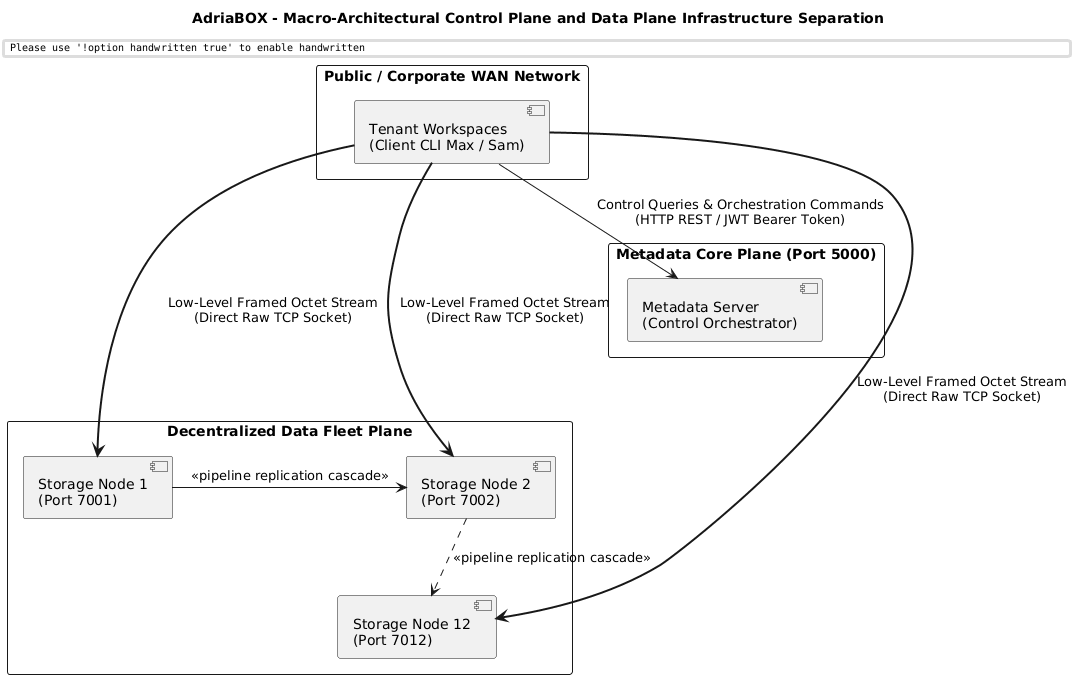
\includegraphics[width=\textwidth]{plantuml/3.1-macro-architecture.png}
    \caption{AdriaBOX Macro-Architectural Control Plane and Data Plane Infrastructure Separation.}
    \label{fig:macro_architecture}
\end{figure}

\subsubsection{Component Network Positioning}
\begin{itemize}
    \item \textbf{Tenant Workspace Instances:} Independent client nodes running inside disparate local area networks or public internet domains.
    \item \textbf{Metadata Server Instance:} Positioned on a central host system or dedicated public machine, exposing an active REST interface over standard network port \texttt{5000}.
    \item \textbf{Decentralized Storage Fleet:} Composed of 12 autonomous server daemons running as isolated network listeners. To prevent hardware-level port binding collisions within single-host emulation contexts, each node is assigned a unique network port index from an explicit, sequential mapping spectrum (ranging from port \texttt{7001} up to port \texttt{7012}).
\end{itemize}

\subsubsection{Service Naming and Component Discovery}
Component mapping and network location identification utilize an explicit configuration matrix. The metadata controller reads environmental configuration declarations to discover active storage target coordinates, tracking parameters including internal cluster host strings, external client entry paths, and raw TCP communication ports. When generating storage plans, the controller serializes these precise connection vectors directly into a client JSON response payload. This design decision makes the client nodes completely independent of complex dynamic domain name service (DNS) lookups or heavy service discovery daemons, resulting in low overhead and direct socket connection capability.

\subsection{Modelling and Static Class Blueprint}
AdriaBOX relies on an object-oriented modeling architecture to isolate responsibilities across decoupled components. The system structure and static object relationships are detailed in the class blueprint in \Cref{fig:class_diagram}.

\begin{figure}[htbp]
    \centering
    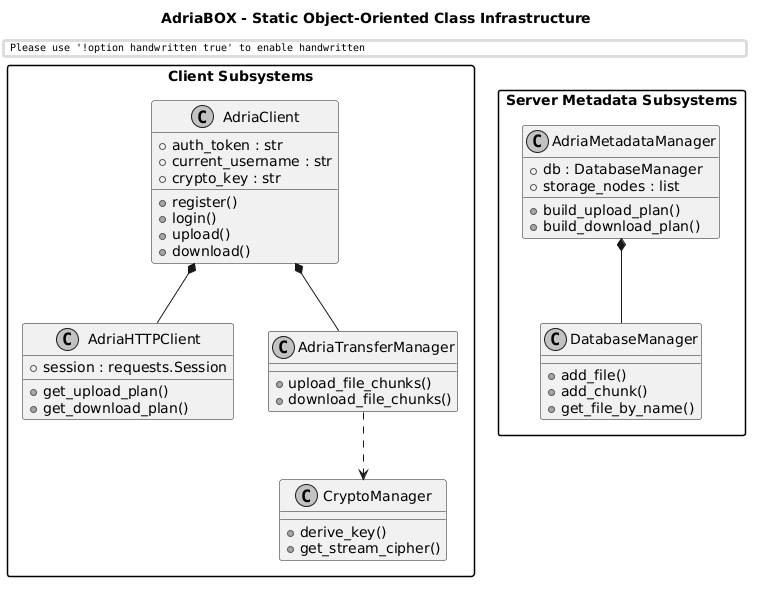
\includegraphics[width=0.9\textwidth]{plantuml/3.2-class-diagram.png}
    \caption{AdriaBOX Static Object-Oriented Class Infrastructure and Module Boundaries.}
    \label{fig:class_diagram}
\end{figure}

\subsubsection{Core Domain Entities}
The system logic operates on three primary structural domain entities:
\begin{itemize}
    \item \textbf{User Tenant Model:} Represents an isolated user account, encapsulating unique system identifiers, validated username strings, administrative access permission flags, and current storage footprint quotas.
    \item \textbf{File Meta-Object:} Tracks virtual assets within the flat S3-style namespace, containing parameters such as global virtual string paths, total sizes in bytes, owner references, and the total logical block allocation count.
    \item \textbf{Logical Chunk Fragment Mapping:} Links an individual block partition index to an explicit list of storage nodes, tracking target block filenames and exact segment byte capacities.
\end{itemize}

\subsubsection{Message Interchange Classification}
The communications flowing through the infrastructure are categorized into three distinct execution types:
\begin{itemize}
    \item \textbf{Control Queries:} Stateless HTTP REST requests dispatched from client machines to browse or check state (e.g., fetching active space metrics or listing directory paths).
    \item \textbf{Orchestration Commands:} Action-oriented instructions that modify state (e.g., initiating login sessions or requesting an authorized upload plan).
    \item \textbf{Low-Level Application Framed Packets:} Customized binary byte-streams sent over raw TCP connections, optimized for streaming data segments between client transfer modules and storage daemons.
\end{itemize}

\subsection{Interaction Patterns and Low-Level Network Framing}
The network engine uses a custom application-layer protocol framing design to handle binary data blocks over raw TCP sockets. Because TCP socket connections provide a continuous stream of unstructured bytes without native message boundary markers, a receiver cannot natively deduce where a control header ends and where raw data payloads begin. AdriaBOX resolves this by building a strict serialization pattern directly into the byte stream. The protocol layout for an upload transaction is detailed in \Cref{fig:tcp_framing}.

\begin{figure}[htbp]
    \centering
    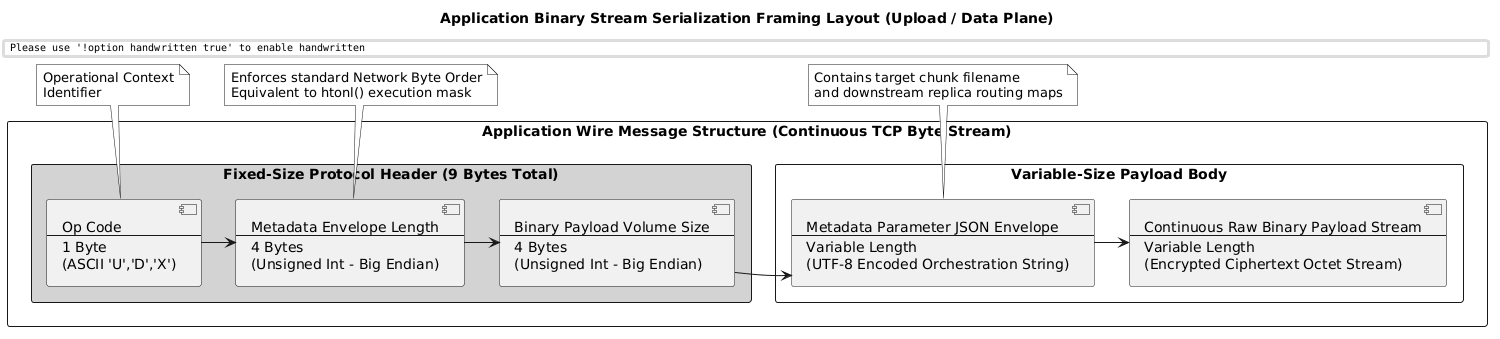
\includegraphics[width=0.95\textwidth]{plantuml/3.3-tcp-framing.png}
    \caption{Application Binary Stream Serialization Framing Layout for Upload Operations.}
    \label{fig:tcp_framing}
\end{figure}

The transmission framing format splits the byte sequence into five distinct operational regions:
\begin{enumerate}
    \item \textbf{Operation Code Indicator (1 Byte):} A single ASCII character specifying the target routine (e.g., character \texttt{'U'} for an upload pipeline, character \texttt{'D'} for a download pull, or character \texttt{'X'} for a physical erasure signal).
    \item \textbf{Metadata Envelope Length (4 Bytes):} An unsigned 32-bit integer, encoded strictly in Big-Endian (Network Byte Order, equivalent to standard \texttt{htonl} C byte ordering). This defines the exact length of the subsequent JSON tracking block.
    \item \textbf{Binary Payload Volume Size (4 Bytes):} An unsigned 32-bit Big-Endian integer that specifies the exact volume size of the streaming data block, preventing connection stalls or buffer overruns.
    \item \textbf{Metadata Parameter JSON Envelope (Variable Length):} A UTF-8 encoded text string containing system orchestration directives, such as the target block filename and an array of downstream replica target node coordinates.
    \item \textbf{Continuous Raw Binary Payload Stream (Variable Length):} The physical chunk segment data, pushed through consecutive micro-packet transfer loops.
\end{enumerate}

\subsubsection{Bit-Level Wire Layout and Memory Alignment Specification}
To satisfy formal network protocol standards, the packet stream layout must be specified bit-by-bit to guarantee deterministic un-packing alignment. \Cref{tab:rfc_wire_format} details the exact byte offsets, data type representations, and bit-level allocation boundaries enforced within the custom \texttt{AdriaTCPStreamer} implementation layers.

\begin{table}[htbp]
\small
\centering
\caption{AdriaBOX Low-Level TCP Wire Layout and Bit Alignment Specification (RFC Style)}
\label{tab:rfc_wire_format}
\vspace{2mm}
\begin{tabularx}{\textwidth}{|c|c|c|l|X|}
\hline
\textbf{Byte Offset} & \textbf{Bit Boundaries} & \textbf{Field Token} & \textbf{Native Data Type} & \textbf{Endianness Order} \\ \hline
\texttt{0x00} & Bits 0--7 & \texttt{Op Code} & 8-bit ASCII Char & Network-Agnostic \\ \hline
\texttt{0x01} & Bits 8--39 & \texttt{Meta Length} & 32-bit Unsigned Int (\texttt{>I}) & Big-Endian (\texttt{Network Byte Order}) \\ \hline
\texttt{0x05} & Bits 40--71 & \texttt{Payload Size} & 32-bit Unsigned Int (\texttt{>I}) & Big-Endian (\texttt{Network Byte Order}) \\ \hline
\texttt{0x09} & Variable & \texttt{Meta Envelope} & UTF-8 Packed JSON String & Stream Byte Array \\ \hline
\texttt{Variable} & Variable & \texttt{Binary Stream} & Raw Octet Byte Sequence & Stream Byte Array \\ \hline
\end{tabularx}
\end{table}

This bit-level mapping enforces rigid structure constraints. By invoking Python's native \texttt{struct.pack('>I', val)} mechanics, the client forces a 4-byte network representation equivalent to building a raw C structural mask with an explicit \texttt{htonl()} conversion wrapper. This design ensures absolute interoperability; an external storage daemon compiled in native C or Go can read the wire layout directly by aligning its un-packing masks with these exact bit offsets.

\subsection{Dynamic System Behaviour and Data Streaming Engine}
To guarantee memory footprint safety and prevent system crashes during large file transfers, the data plane streaming engine runs a strict resource management model. The step-by-step memory allocation and byte copy flow within the Linux user-space boundary are formalized in \Cref{fig:data_plane_streaming}.

\begin{figure}[htbp]
    \centering
    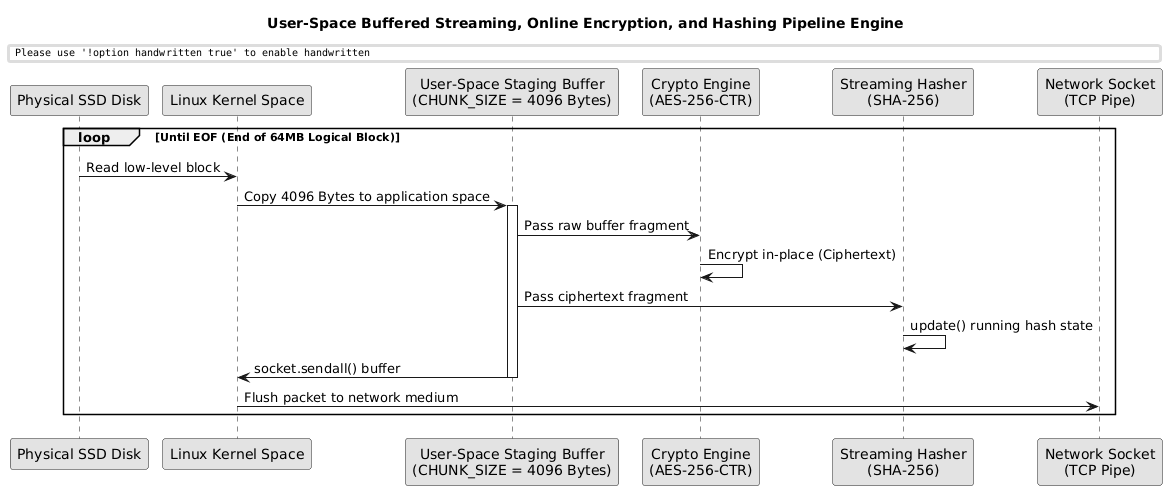
\includegraphics[width=\textwidth]{plantuml/3.4-data-plane-streaming.png}
    \caption{User-Space Buffered Streaming, Online Encryption, and Hashing Pipeline Engine.}
    \label{fig:data_plane_streaming}
\end{figure}

The storage daemons and client modules enforce a bounded memory execution model. Instead of reading an entire 64MB logical block into memory using a single large I/O call, the transfer manager sets up a constant 4096-Byte user-space staging buffer. The low-level execution loop follows a strict sequential pipeline:
\begin{enumerate}
    \item The client initiates an iterative loop, pulling small data blocks from disk storage via kernel-space read buffers into the application space staging buffer.
    \item The 4KB data snippet passes through the cryptography engine, where an inline AES-256-CTR transformation modifies the byte array in-place, avoiding extra memory copies.
    \item The mutated buffer is passed directly to the streaming hashing module, which updates its running state to compute the SHA-256 cryptographic signature on the fly.
    \item A socket system call immediately flushes the 4KB buffer down the network pipe to the target storage node daemon.
\end{enumerate}
This processing model ensures that memory usage during file transfers remains static at $O(1)$ complexity, requiring exactly 4 Kilobytes of operational RAM regardless of the total file capacity.

\subsubsection{Multi-Threaded Node Concurrency and Direct I/O Isolation}
To sustain concurrent data plane transfers without experiencing network blocking or memory page corruption, the backend worker nodes virtualize client socket requests via an asynchronous thread pool architecture. The internal process-threading model executed within each storage node daemon is formalized in \Cref{fig:storage_threading_concurrency}.

\begin{figure}[htbp]
    \centering
    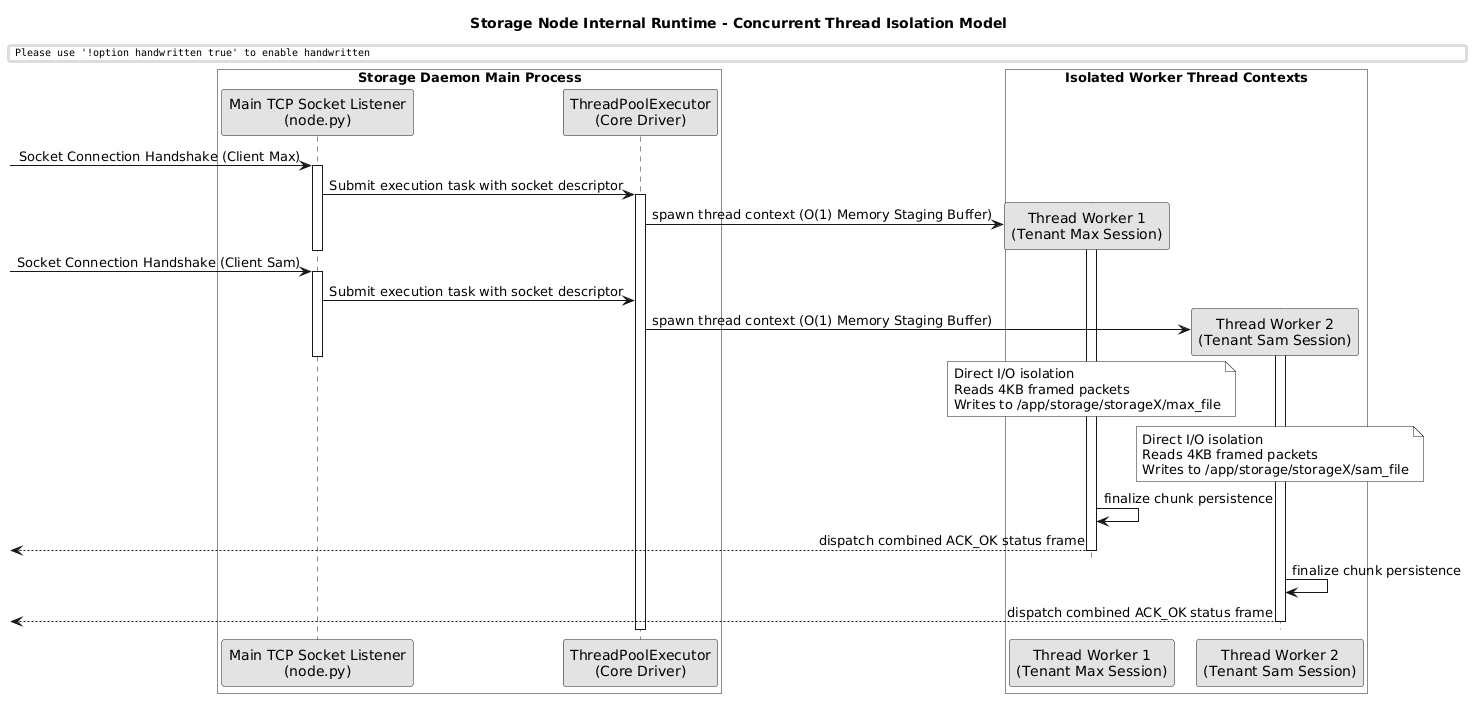
\includegraphics[width=0.95\textwidth]{plantuml/3.5-storage-threading.png}
    \caption{Storage Node Internal Thread Allocation and Direct Multi-Tenant Process Isolation Map.}
    \label{fig:storage_threading_concurrency}
\end{figure}

When multiple client processes open simultaneous connections to a node's interface, the main thread's \texttt{socket.accept()} loop hands off the raw descriptor to a centralized \texttt{ThreadPoolExecutor} context. This subsystem isolates each connection transaction within an independent worker thread lifecycle:
\begin{itemize}
    \item \textbf{Execution Context Separation:} Each active thread instantiates isolated instances of the wire formatting parser, allocating a separate 4096-Byte staging buffer in user-space RAM. Memory addresses do not cross thread barriers, preventing dirty read-write data states across concurrent streams.
    \item \textbf{Direct I/O Boundary Isolation:} The worker thread tracks its own file descriptor variables, performing concurrent writes to different, un-linked target block storage partitions on the host filesystem disk.
\end{itemize}
This multi-threaded architecture allows a single storage node daemon container to ingest multi-gigabyte blocks from multiple distinct users simultaneously, maintaining high-throughput cluster performance while keeping the operational resource footprint flat.

\subsection{Data Persistence and Multi-Tenant Query Scope}
The control plane isolates multi-tenant environments by applying strict security filters to database queries. When a client requests a file listing, the metadata controller intercepts the request and determines the query scope based on the user's role context, as detailed in \Cref{fig:admin_user_bifurcation}.

\begin{figure}[htbp]
    \centering
    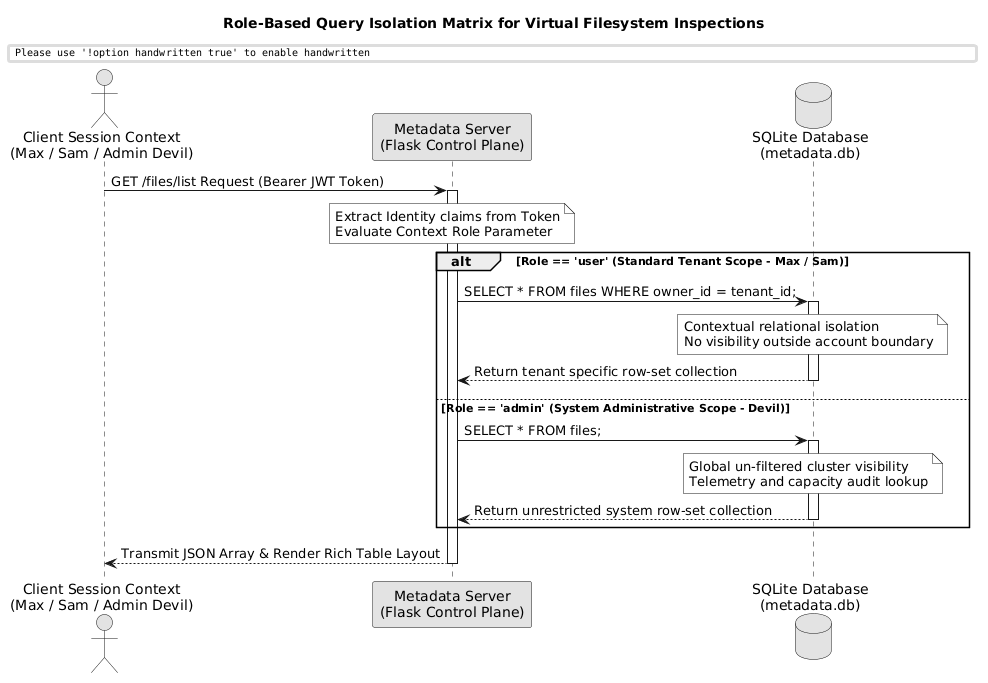
\includegraphics[width=0.95\textwidth]{plantuml/3.6-admin-user-bifurcation.png}
    \caption{Role-Based Query Isolation Matrix for Virtual Filesystem Inspections.}
    \label{fig:admin_user_bifurcation}
\end{figure}

The metadata database relies on a strictly relational SQL schema to maintain system state:
\begin{itemize}
    \item \textbf{\texttt{users} Table:} Stores unique tenant identifiers, system usernames, secure authentication hashes, active system roles, and creation timestamps.
    \item \textbf{\texttt{files} Table:} Records global file paths, file sizes, block counts, creation dates, and owner ID references to enforce multi-tenant separation.
    \item \textbf{\texttt{chunks} Table:} Maps individual file segment blocks to their primary storage node locations, tracking block filenames and chunk sizes.
\end{itemize}

Query scoping handles permissions via role-based access logic:
\begin{itemize}
    \item \textbf{Standard User Scope:} Queries are bound to the tenant's context via explicit SQL constraints (e.g., appending a restrictive \texttt{WHERE owner\_id = user\_id} clause). This ensures users can only view or interact with their own assets.
    \item \textbf{Administrative Scope:} Queries run without tenant-level filters, giving administrators broad visibility into system metrics, aggregate disk usage, and multi-tenant user lists.
\end{itemize}

\subsection{Fault Tolerance and Resilient Pipeline Replication}
AdriaBOX provides data redundancy and cluster availability using a synchronous pipeline replication strategy. When writing file chunks to the data plane, data flows down a coordinated node cascade to guarantee safety across failure domains, as shown in \Cref{fig:upload_pipeline}.

\begin{figure}[htbp]
    \centering
    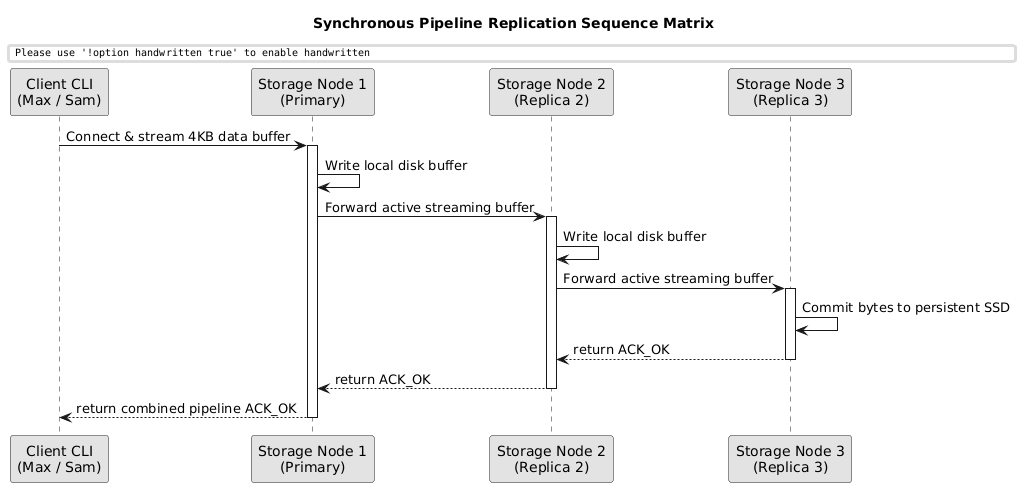
\includegraphics[width=0.95\textwidth]{plantuml/3.7-upload-pipeline.png}
    \caption{Synchronous Pipeline Replication Sequence and Cascading Verification Verification Flow.}
    \label{fig:upload_pipeline}
\end{figure}

\subsubsection{Synchronous Redundancy Chain}
The metadata master uses a Chained Round-Robin scheduling algorithm to calculate three unique node addresses for each block. Data flows down the chain sequentially:
$$\text{Replication Cascade: } \text{Client} \longrightarrow \text{Node}_{\text{Primary}} \longrightarrow \text{Node}_{\text{Replica 2}} \longrightarrow \text{Node}_{\text{Replica 3}}$$
The data streaming and write confirmations flow in opposing directions:
\begin{enumerate}
    \item The client streams the 4KB data buffers directly to the primary storage node.
    \item As the primary node receives the data, it copies the buffers to its local disk while concurrently forwarding the stream to the second node in the pipeline.
    \item The second node copies the bytes locally and forwards them to the final replica node.
    \item Write confirmations flow back up the chain in reverse order ($\text{Node}_3 \rightarrow \text{Node}_2 \rightarrow \text{Node}_1 \rightarrow \text{Client}$).
    An upload is only flagged as successful when the primary node receives a valid confirmation from the downstream replicas, ensuring the block is safely written across three separate failure domains.
\end{enumerate}

\subsubsection{Client-Side Failover Architecture}
To remain online during node crashes or network partitions, the client transfer manager uses an automated client-side failover loop, as detailed in \Cref{fig:download_failover}.

\begin{figure}[htbp]
    \centering
    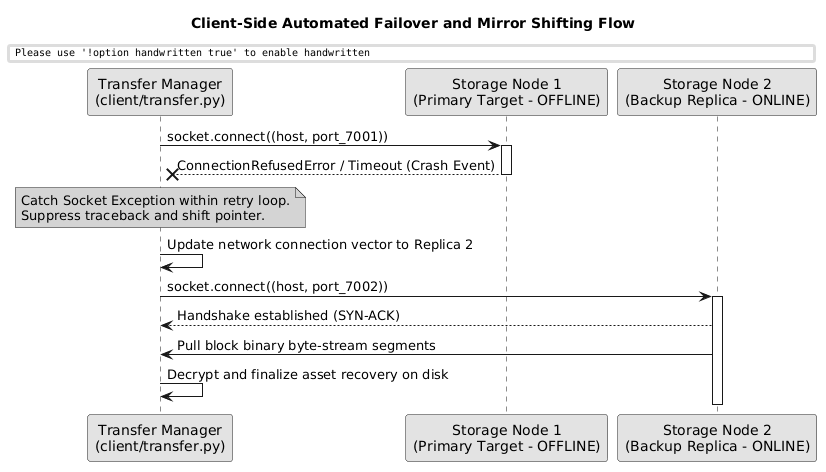
\includegraphics[width=0.95\textwidth]{plantuml/3.8-download-failover.png}
    \caption{Client-Side Automated Failover and Mirror Shifting Flow during Node Failure.}
    \label{fig:download_failover}
\end{figure}

When a download transaction begins, the client fetches an orchestration plan containing the primary location and all replica addresses for each chunk. If the primary node is offline or times out, the transfer manager catches the exception, logs a warning to the interface, and automatically shifts its connection pointer to the next backup replica address in the plan. This failover loop runs entirely in user-space, maintaining system availability without adding extra query overhead to the central metadata database.

\subsection{Availability and CAP Strategy}
The system is explicitly designed as a \textbf{CP-focused infrastructure} (Consistency and Partition Tolerance) under the CAP Theorem framework. It prioritizes absolute data correctness and metadata validity over uncoordinated uptime. If a network partition isolates a cluster segment, the system handles state conflicts through two strict design rules:
\begin{itemize}
    \item \textbf{Central Control Authority:} All metadata modifications must clear through the authoritative central controller. If a client is partitioned away from the master node, it cannot write data directly to the storage nodes, preventing split-brain or divergent metadata scenarios.
    \item \textbf{Atomic Transaction Abort:} If a network partition interrupts a replication pipeline midway through a file transfer, the transaction aborts. The primary node returns an error to the client, preventing partial writes or uncoordinated block states.
\end{itemize}

\subsection{Security and Access Isolation}
Security boundaries are enforced using strict authorization layers and client-side encryption routines:

\subsubsection{Session Authentication and Token Isolation}
Users register and authenticate credentials through the central control interface. Upon a successful login, the server issues a stateful JSON Web Token (JWT) signed with a secure server key. The client CLI caches this token locally and appends it to the authorization headers of all subsequent control plane requests, keeping the system's control APIs secure.

\subsubsection{Zero-Knowledge Cryptographic Isolation}
Data privacy is protected using a Zero-Knowledge encryption model. When a user authenticates, the client CLI reads the raw password and uses the PBKDF2 function with 100,000 hashing iterations to derive a secure 256-bit AES key. This key is isolated within the local client workspace and is never transmitted over the network or exposed to the master node or storage cluster. Data blocks are encrypted on the fly using the AES-256-CTR stream cipher before leaving the client machine, ensuring that data stored on the cluster remains secure and unreadable to unauthorized parties or system administrators.

\subsection{Dual-Layer Cryptographic Architecture and Zero-Knowledge Paradigm}
\label{sub:crypto_architecture}

To satisfy the stringent privacy and isolation metrics defined in \Cref{sec:requirements}, AdriaBOX implements a dual-layer cryptographic framework. This architecture clean cuts the boundaries between transit-layer wire protection and persistent asset confidentiality, enforcing a strict \textbf{Zero-Knowledge paradigm} where the cloud infrastructure provider possesses zero visibility into the tenant's plaintext binary payload.

\subsubsection{Control Plane Protection: Transport-Layer Security (HTTPS)}
All administrative, authentication, and metadata orchestration pathways operating over the Control Plane (directed from the Client CLI to the Flask Metadata Server) utilize standard \textbf{Transport-Layer Security (TLS/HTTPS)} in a production environment. This mechanism encapsulates standard HTTP REST JSON structures inside an asymmetric/symmetric handshake envelope (Layer 5 of the OSI stack). While HTTPS successfully mitigates middleman eavesdropping, packet tampering, and session hijacking during network transit, it terminates at the edge of the Control Plane: the Metadata Server decrypts the incoming TLS packet to evaluate and execute the business logic. Consequently, transport-layer encryption alone is mathematically insufficient to guarantee complete data privacy inside a multi-tenant storage cluster.

\subsubsection{Data Plane Isolation: Client-Side Zero-Knowledge Encryption}
To ensure that files remain completely unreadable even to malicious system administrators or compromised storage hardware, the Data Plane enforces an end-to-end symmetric encryption model executing exclusively within the local host user-space boundary.
\begin{enumerate}
    \item \textbf{Deterministic Key Derivation (PBKDF2HMAC):} When a user triggers an execution session via the CLI, the local runtime intercepts the plain password. To prevent cryptographic key collision attacks—where distinct users utilizing identical weak passwords yield equivalent keys—the system feeds the password into the PBKDF2HMAC algorithm. The unique system \texttt{username} is systematically injected as a deterministic cryptographic \textit{salt}, stretched over exactly 100,000 computation iterations using the SHA-256 hashing primitive. The resulting 256-bit (32-byte) key is safely isolated inside the client memory page structures.
    \item \textbf{In-Place Stream Ciphering (AES-256-CTR):} Prior to logical block striping and socket broadcasting, data flows through the local cryptographic engine. The system instantiates an Advanced Encryption Standard (AES) block cipher operating in Counter (CTR) mode. CTR mode virtualizes the block cipher into a continuous stream cipher by computing an invariant keystream bit-by-bit, eliminating the architectural requirement for memory padding overhead. To defeat cryptographic patterns, a unique 16-byte cryptographic Nonce (Initialization Vector) is calculated for each individual chunk by running a SHA-256 digest over the target chunk filename.
\end{enumerate}

The structural interaction boundaries detailing exactly where the Transport-Layer Security (HTTPS) and the local Zero-Knowledge Engine (\texttt{crypto.py}) operate across the network plane are formalized in \Cref{fig:cryptographic_boundaries}.

\begin{figure}[htbp]
    \centering
    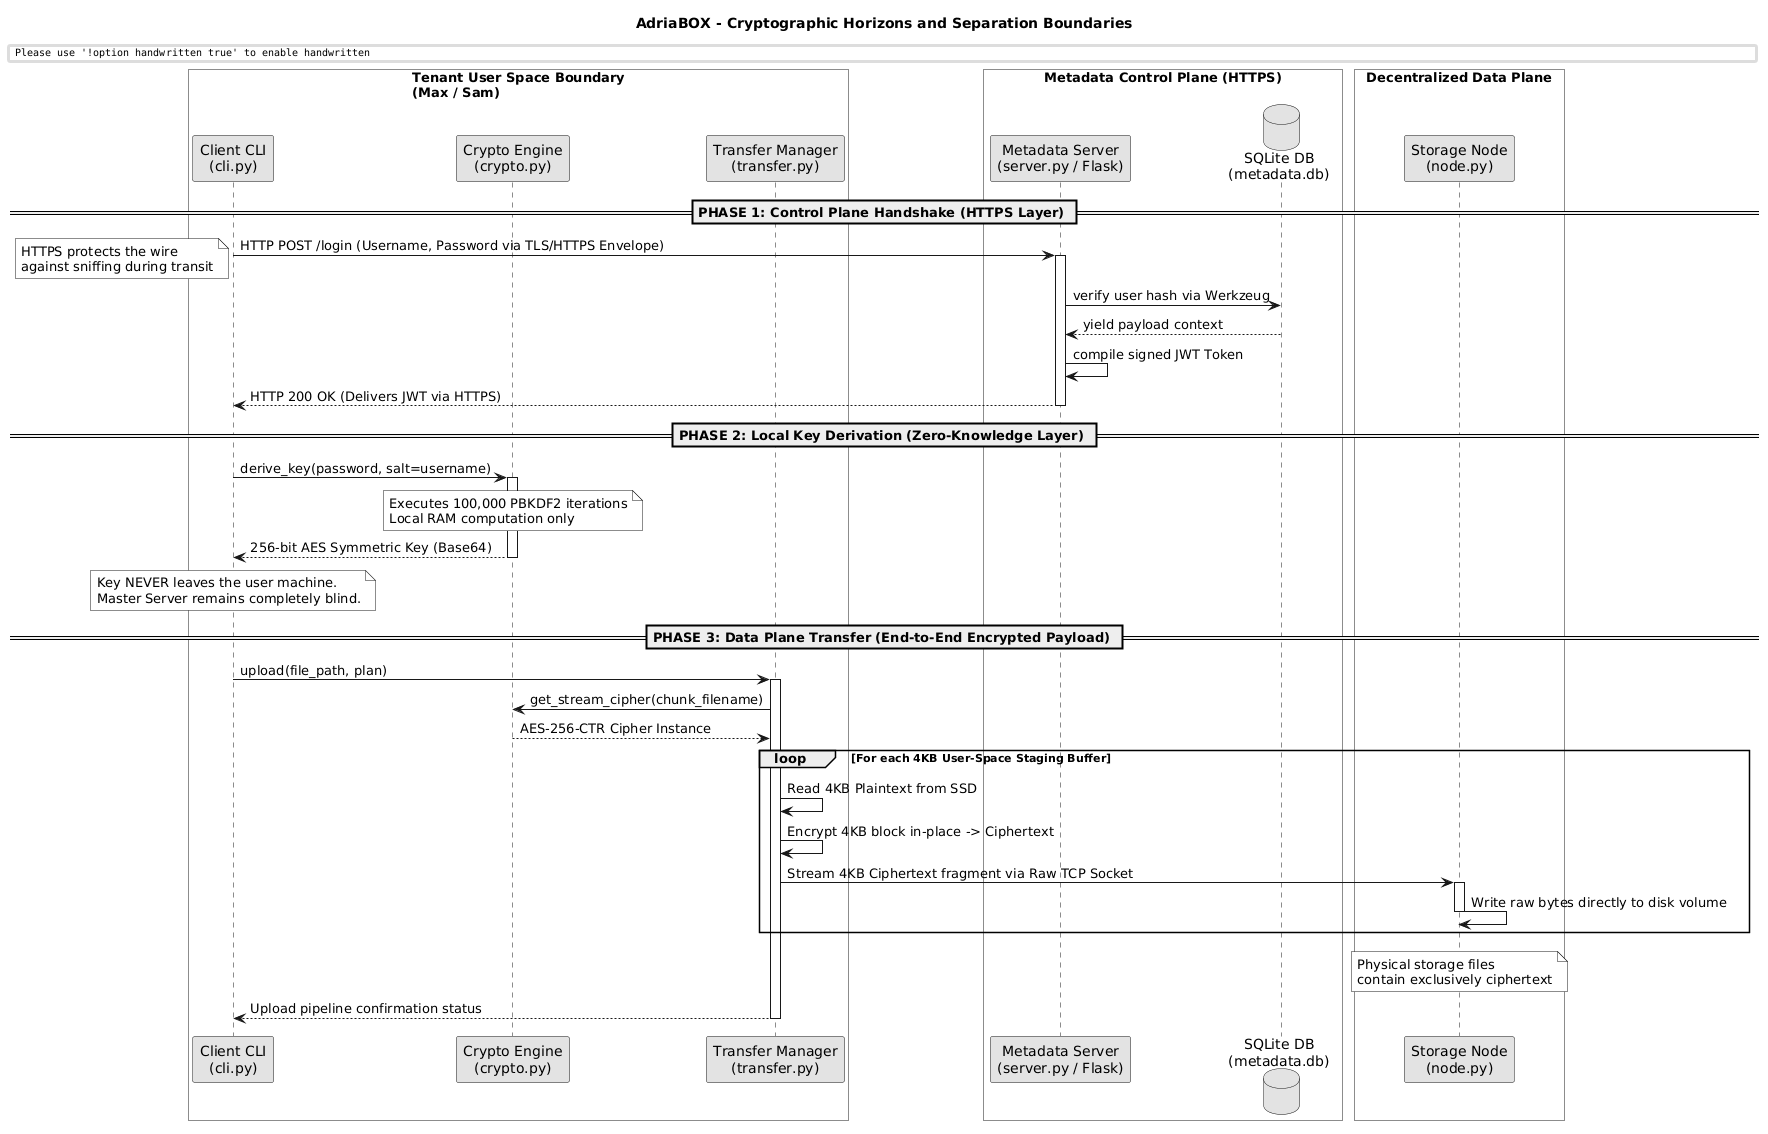
\includegraphics[width=\textwidth]{plantuml/3.9-cryptographic-boundaries.png}
    \caption{AdriaBOX Dual-Layer Cryptographic Boundary and Processing Horizons Map.}
    \label{fig:cryptographic_boundaries}
\end{figure}
% --- CHAPTER 3: DESIGN ---
All administrative, authentication, and metadata orchestration pathways operating over the Control Plane (directed from the Client CLI to the Flask Metadata Server) utilize standard \textbf{Transport-Layer Security (TLS/HTTPS)} in a production environment[cite: 1668]. This mechanism encapsulates standard HTTP REST JSON structures inside an asymmetric/symmetric handshake envelope (Layer 5 of the OSI stack)[cite: 1669]. While HTTPS successfully mitigates middleman eavesdropping, packet tampering, and session hijacking during network transit, it terminates at the edge of the Control Plane: the Metadata Server decrypts the incoming TLS packet to evaluate and execute the business logic[cite: 1670]. Consequently, transport-layer encryption alone is mathematically insufficient to guarantee complete data privacy inside a multi-tenant storage cluster[cite: 1671].

\subsubsection{Data Plane Isolation: Client-Side Zero-Knowledge Encryption}
To ensure that files remain completely unreadable even to malicious system administrators or compromised storage hardware, the Data Plane enforces an end-to-end symmetric encryption model executing exclusively within the local host user-space boundary[cite: 1672].
\begin{enumerate}
    \item \textbf{Deterministic Key Derivation (PBKDF2HMAC):} When a user triggers an execution session via the CLI, the local runtime intercepts the plain password[cite: 1673]. To prevent cryptographic key collision attacks—where distinct users utilizing identical weak passwords yield equivalent keys—the system feeds the password into the PBKDF2HMAC algorithm[cite: 1674]. The unique system \texttt{username} is systematically injected as a deterministic cryptographic \textit{salt}, stretched over exactly 100,000 computation iterations using the SHA-256 hashing primitive[cite: 1675]. The resulting 256-bit (32-byte) key is safely isolated inside the client memory page structures[cite: 1676].
    \item \textbf{In-Place Stream Ciphering (AES-256-CTR):} Prior to logical block striping and socket broadcasting, data flows through the local cryptographic engine[cite: 1677]. The system instantiates an Advanced Encryption Standard (AES) block cipher operating in Counter (CTR) mode[cite: 1678]. CTR mode virtualizes the block cipher into a continuous stream cipher by computing an invariant keystream bit-by-bit, eliminating the architectural requirement for memory padding overhead[cite: 1679]. To defeat cryptographic patterns, a unique 16-byte cryptographic Nonce (Initialization Vector) is calculated for each individual chunk by running a SHA-256 digest over the target chunk filename[cite: 1680].
\end{enumerate}

The structural interaction boundaries detailing exactly where the Transport-Layer Security (HTTPS) and the local Zero-Knowledge Engine (\texttt{crypto.py}) operate across the network plane are formalized in \Cref{fig:3.9-cryptographic-boundaries}[cite: 1681].

\begin{figure}[htbp]
    \centering
    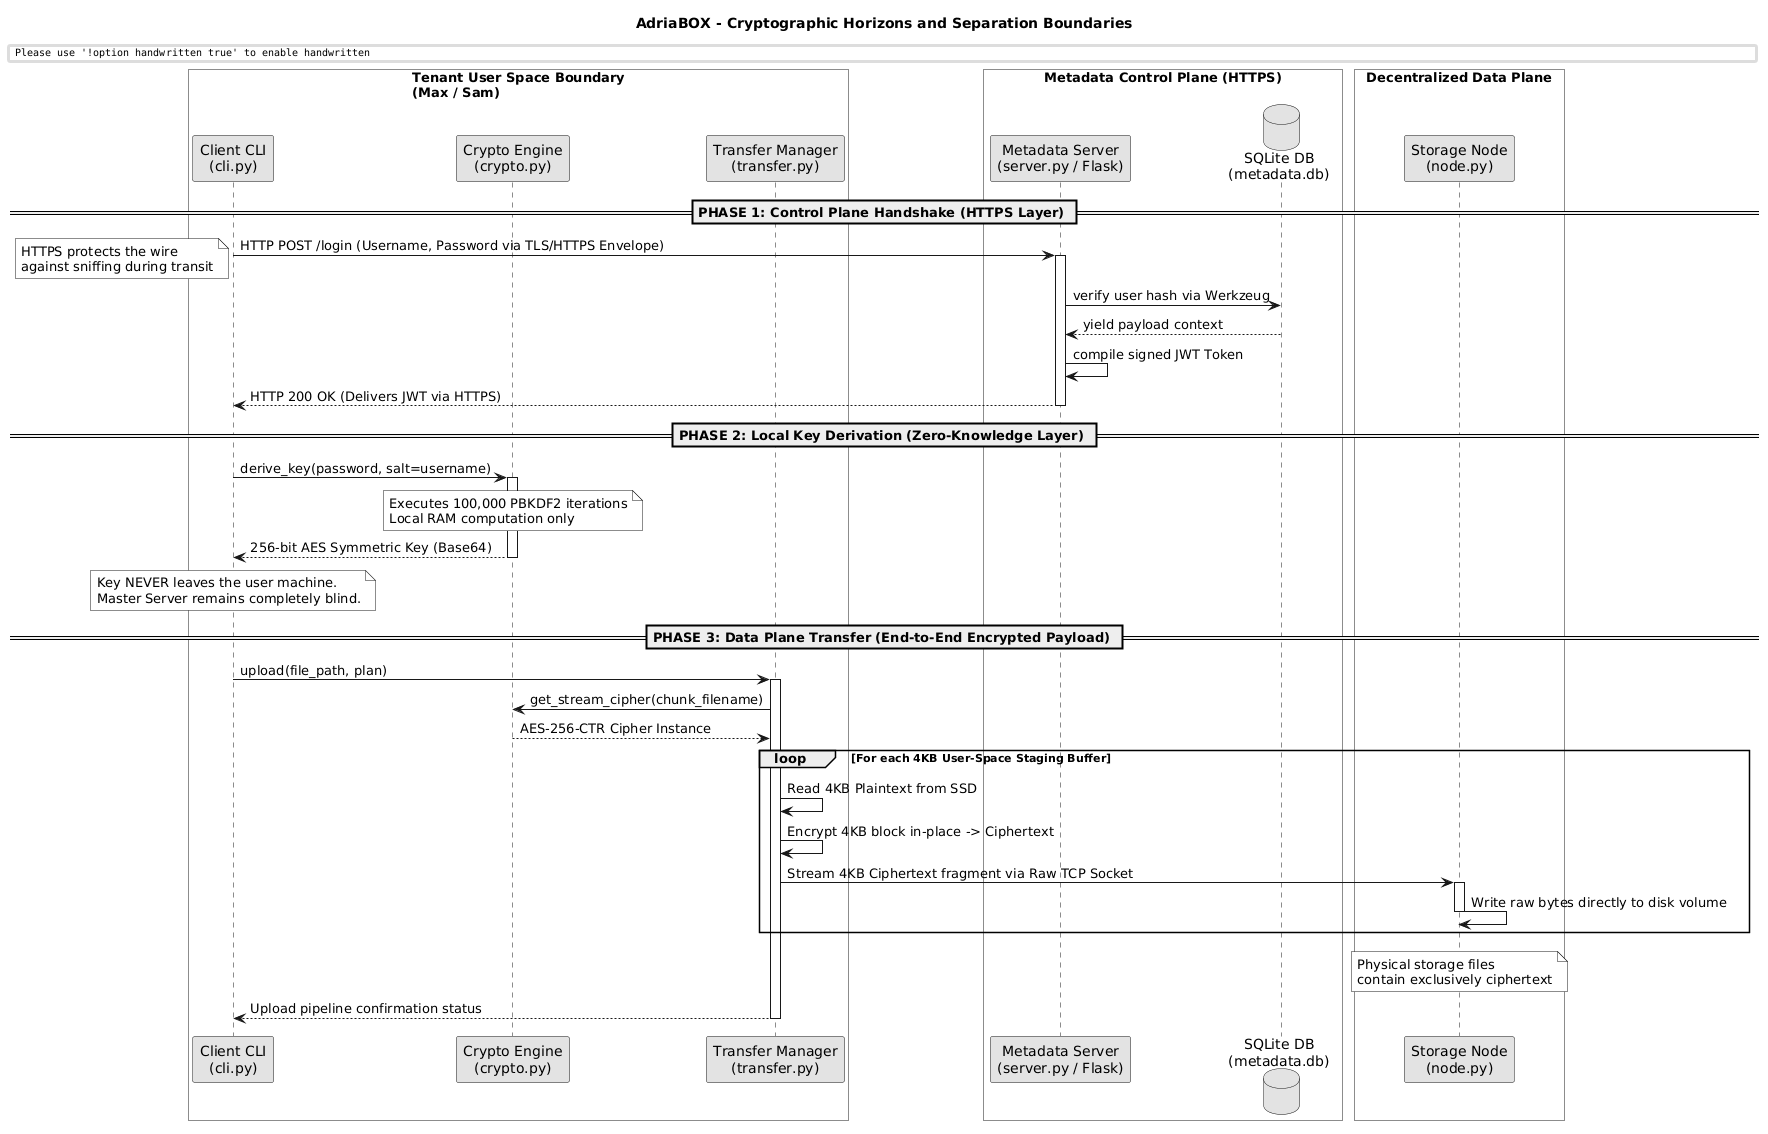
\includegraphics[width=\textwidth]{plantuml/3.9-cryptographic-boundaries.png}
    \caption{AdriaBOX Dual-Layer Cryptographic Boundary and Processing Horizons Map.}
    \label{fig:3.9-cryptographic-boundaries}
\end{figure}